\begin{figure}[t]
\centering
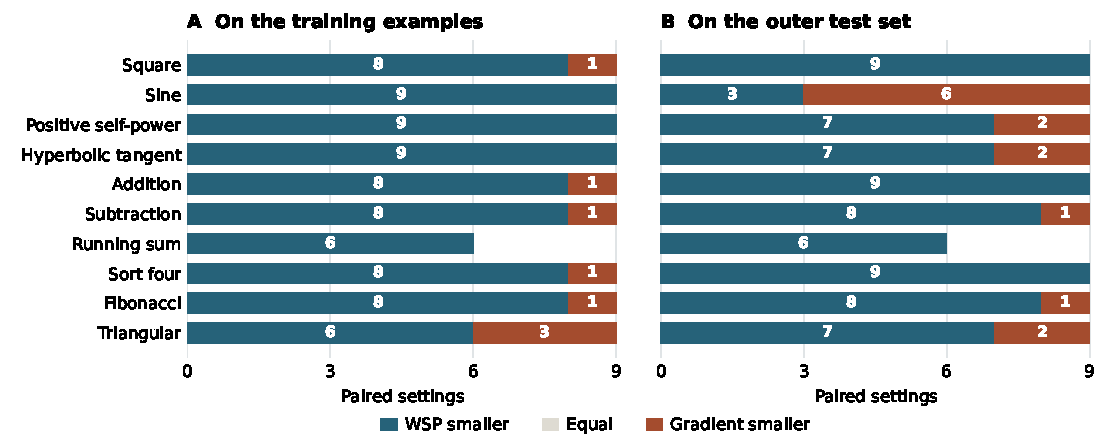
\includegraphics[width=\linewidth]{figure1.pdf}
\caption{The first WSP reply given examples only and the Adam--BFGS gradient fit start from the same weights on the same task and architecture. Each bar counts how often one method's endpoint has smaller error or the two unrounded recorded errors agree. Even a very small strict difference is counted. Panel A uses their common loss on the labeled training examples. Panel B uses raw root mean squared error (RMSE) on held-out outer inputs in each target's own units. Each task contributes three sizes with three starts, except running sum with two sizes and three starts. Every listed setting has a certified nonconvex training objective.}\label{fig:paired_endpoints}
\end{figure}
